\documentclass{article}

\usepackage[margin=1in]{geometry}
\usepackage{amsfonts}
\usepackage{amssymb}
\usepackage{mathtools}
\usepackage{graphicx}
\graphicspath{ {./../../} }
\linespread{2}

\begin{document}

\title{	CMSC 471 -- Project 2\\ 
	Local Searches}
\author{Jeremy Aguillon}

\maketitle

\newpage

\section{Basic Hillclimbing}

\begin{figure}
	\centering
	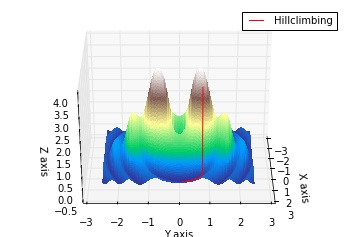
\includegraphics[scale=1]{hillclimbingSearchFinal.jpg}
	\caption{A successful Hillclimbing search path}
	\label{fig:hillclimbingSearchFinal}
\end{figure}

For the first part of this assignment, I have implemented a basic hillclimbing searching algorithm. This works by simply finding the first direction that leads the function to have a lower minimum and performs the same search on that new area. I found the best way to do this was to calculate the current position, and iterate through a while loop and update the value each time the loop iterates. I found a reasonable step size for this algorithm to be .05 when searching the space from -2.5 to 2.5. This algorithm however is very prone to getting stuck in local minimums and can sometimes give very misleading results if this occurs. Figure \ref{fig:hillclimbingSearchFinal} shows a successful search that my algorithm took through the given function. It began at a very high point in the function and dropped straight down to the bottom as hillclimbing should. Overall this was the simplest and least effective algorithm.

\section{Hillclimbing With Random Restarts}

\begin{figure}
	\centering
	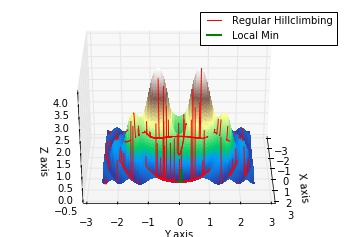
\includegraphics[scale=1]{HCWRRSearchFinal.jpg}
	\caption{A successful Hillclimbing with random restarts search path}
	\label{fig:HCWRRSearchFinal}
\end{figure}

The next algorithm takes the previous algorithm and adds accuracy by repetition. Hillclimbing with random restarts takes the original hillclimbing algorithm and runs it many times from different points in the search space to avoid local minimum and gives the user a much better idea of the global minimum of the space. To do this I chose a random space, called the hillclimbing algorithm on that space, chose another random space, called hillclimbing on that space and kept track of the lowest minimum that all the hillclimbings have found. I found that it is better to have more restarts to I chose to run hillclimbing 100 times, with the same .05 step, before returning the lowest minimum. This algorithm is less likely to get all searches caught in local minimums and will have a much larger range to get the actual global minimum. Figure \ref{fig:HCWRRSearchFinal} shows the space being searched by 100 hillclimbing searches and the green line indicates the lowest minimum that they found.

\section{Simulated Annealing}

\begin{figure}
	\centering
	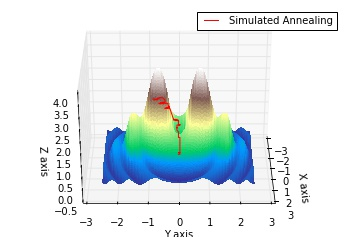
\includegraphics[scale=1]{simAnnealSearchFinal.jpg}
	\caption{A successful Simulated Annealing search path}
	\label{fig:simAnnealSearchFinal}
\end{figure}	


The final algorithm is simulated annealing, which is an algorithm based on the cooling of metal. It uses a cooling property that starts very hot and cools down to imitate this metal. The hotter the state of the algorithm is, the more likely it will make a bad move. By allowing the algorithm to make a bad move, it will be able to escape local minimums and have a better chance at finding the global minimum. To code this I initialized the cooling rate to .95 so it cools slowly and gets a better look at the graph. The step size was .25 so it could explore more of the graph with each step than hillclimbing. After initializing these variables, I put the calculations in a while loop for each step until the temperature reaches .0001, allowing the loop to run for many iterations. Once inside the loop my algorithm calculates a move in each direction and picks one randomly. If the move moves it closer to a minimum, then it takes it, otherwise it is put into the probability function that has a higher likelihood of accepting a bad move, the hotter the temperature is. Figure \ref{fig:simAnnealSearchFinal} shows the function working properly where it started from a high point in the graph and took some lateral and bad moves at the beginning, but moved more towards hillclimbing as it went down the graph and the temperature cooled.

\section{Results}

\newpage

I ran each algorithm once to produce a graphical depiction of the path each search takes. Then I ran each algorithm an additional 100 times to calculate some statistics to compare them to one another. In Figure \ref{averageData} are the results of one run through of 100 tests on the given graph. I calculated the average min with $$\frac{(\sum_{}^{} min)}{100} $$ and	average time was calculated with $$\frac{\sum_{}^{} (endTime - startTime) }{100}$$  Unique mins were found by setting the decimal precision to 4 decimal places for each local min and putting them in an array and finding the length of that array after 100 runs.

	\begin{figure}
		\centering
		\begin{tabular}{|l|c|c|c|} 
			\hline 
			& Hillclimbing & HC W/ Restarts & Simulated Annealing \\
			\hline
			Avg Min & -0.116546172004 & -0.150259158849 & -0.117060168829 \\
			Avg Time & 0.004872303009033203 & 0.39496626853942873 & 0.05540627479553223 \\
			Unique Mins & 88 & 2 & 94 \\
			\hline
		\end{tabular}
		\caption{Table showing statistics from 100 runs from each algorithm}
		\label{averageData}
	\end{figure}

Shown by Figure \ref{averageData}, hillclimbing with random restarts consistently finds the lowest minimum by about .04 units, with Hillclimbing and Simulated Annealing finding similar results but not as good. Hillclimbing with restarts also is much more precise than either of the other searches because of the restarts and is precise enough to find only 2 unique keys to the fourth decimal precision after 100 runs, while the other two are closer to 100 keys. However, although Hillclimbing with restarts does perform the best, it does take the longest by quite a bit.  




\end{document}